\documentclass[11pt]{article}

\usepackage[margin=1in]{geometry}
\usepackage{graphicx}
\usepackage{booktabs}
\usepackage{amsmath}
\usepackage{amssymb}
\usepackage{hyperref}
\usepackage{natbib}
\usepackage{caption}
\usepackage{subcaption}
\usepackage{xcolor}

\hypersetup{colorlinks=true, linkcolor=blue, citecolor=blue, urlcolor=blue}

\title{Does the Model Know Why?\\
A Failure-Mode Cross-Checking Protocol for Verifying\\
SHAP Explanations in Multi-Mechanism Predictive Maintenance}

\author{
  Koshik Debanath \\
  \small \texttt{koshik.debanath@gmail.com}
}

\date{}

\begin{document}
\maketitle

\begin{abstract}
Post-hoc explanation methods such as SHAP are routinely applied to predictive-maintenance
classifiers, but the resulting attributions are rarely checked against anything beyond the
analyst's intuition. We use a property of the AI4I~2020 predictive maintenance dataset that is
usually discarded: its binary \texttt{Machine failure} label is the logical OR of five
independently defined failure mechanisms (tool wear, heat dissipation, power, overstrain, and a
random failure with no physical cause), each with an exact, published triggering rule. We train an
imbalance-aware gradient-boosted classifier on the composite label only -- withholding the five
sub-labels from the feature set entirely -- and then use the sub-labels purely as a post-hoc audit:
for each mechanism, we compute the model's mean absolute SHAP attribution restricted to the rows
where that mechanism fired, and check whether the top attributed feature matches the mechanism's
known physical cause. The random-failure mechanism, which by construction has no learnable
predictor, serves as a negative control. Across five mechanisms, our tuned XGBoost model
(precision~1.00, recall~0.82, F1~0.90 on the held-out failure class) attributes each real mechanism
to its correct physical cause and shows no dominant feature for the random mechanism. We argue this
cross-checking protocol -- using a dataset's own latent causal substructure as a faithfulness probe,
rather than constructing synthetic ground truth for the purpose -- generalizes to any
predictive-maintenance setting where a coarse target is known to aggregate several distinct,
partially-labeled failure modes, which is the common case in industrial practice.
\end{abstract}

\section{Introduction}

Predictive maintenance (PdM) models are increasingly built with gradient-boosted trees or neural
networks and explained after the fact with SHAP \citep{lundberg2017shap}. The explanation is
typically presented as evidence that the model ``makes sense'' -- a beeswarm plot, a bar chart of
global feature importance -- but is rarely checked against an independent source of truth about
\emph{why} the underlying process actually failed. This is a meaningful gap: a model can achieve
strong discriminative performance while keying off a spurious correlate of failure rather than the
mechanism itself, and a plausible-looking SHAP plot will not by itself reveal the difference
\citep{vollert2024survey}.

The AI4I~2020 dataset \citep{matzka2020explainable} offers an unusual opportunity to close this gap
without constructing anything artificial for the purpose. Its target, \texttt{Machine failure}, is
by design the logical OR of five independent sub-conditions -- tool wear failure (TWF), heat
dissipation failure (HDF), power failure (PWF), overstrain failure (OSF), and a random failure
(RNF) that fires with fixed probability regardless of process state. Each of the first four has an
exact, published closed-form trigger (Table~\ref{tab:mechanisms}); RNF has none. Critically, a model
trained to predict \texttt{Machine failure} is never given these five labels -- it only ever sees
the OR of them. This is exactly the situation faced in real industrial settings, where a single
``needs maintenance'' flag is often an aggregate of several distinct root causes that are logged
separately (or not logged at all) but never exposed to the model as a training signal.

This gives us a natural faithfulness probe: after training on the composite label alone, we can go
back and ask, for the subset of rows where a specific mechanism actually fired, whether the model's
SHAP attributions concentrate on the feature that mechanism's own definition implicates. If they do
not, that is a warning sign that the classifier is exploiting a different, possibly spurious,
correlate. If RNF -- which has no real cause -- shows no dominant attributed feature, that is a
sanity check that the method is not simply finding \emph{something} to blame in every subgroup by
construction.

\paragraph{Contributions.}
\begin{enumerate}
  \item An imbalance-aware benchmark of seven model families (Logistic Regression, SVM, $k$-NN,
    Decision Tree, Random Forest, XGBoost, and a small PyTorch MLP) on AI4I~2020, with a
    resampling-technique bake-off (SMOTE vs.\ Borderline-SMOTE vs.\ ADASYN), hyperparameter and
    decision-threshold tuning, and 5-fold cross-validation.
  \item A lightweight cross-checking protocol that uses a dataset's own latent, partially-labeled
    causal substructure -- rather than purpose-built synthetic ground truth -- to audit whether a
    trained model's SHAP explanations are faithful to the real generating mechanism, including a
    built-in negative control.
  \item An empirical demonstration that a well-tuned XGBoost classifier passes this audit on all
    five mechanisms of AI4I~2020, and a discussion of what a failed audit would look like and how
    the protocol generalizes to other multi-mechanism PdM datasets.
\end{enumerate}

\begin{table}[htbp]
\centering
\caption{The five failure mechanisms underlying \texttt{Machine failure} in AI4I~2020
\citep{matzka2020explainable}. Only the composite OR label is ever shown to the model; the
individual triggers are withheld from training and used only for the audit in
Section~\ref{sec:crosscheck}.}
\label{tab:mechanisms}
\begin{tabular}{@{}llp{7cm}r@{}}
\toprule
Code & Name & Trigger condition & Count \\
\midrule
TWF & Tool wear failure & tool wear falls in a randomly assigned 200--240\,min window & 46 \\
HDF & Heat dissipation failure & (process temp.\ $-$ air temp.) $< 8.6$\,K \textbf{and} rpm $< 1380$ & 115 \\
PWF & Power failure & torque $\times$ rpm (rad/s) outside $[3500\text{W}, 9000\text{W}]$ & 95 \\
OSF & Overstrain failure & tool wear $\times$ torque exceeds a type-specific limit (11/12/13k) & 98 \\
RNF & Random failure & fixed 0.1\% chance, independent of all process variables & 19 \\
\bottomrule
\end{tabular}
\end{table}

\section{Related Work}

\citet{matzka2020explainable} introduced the AI4I~2020 dataset alongside a LIME-based
illustration of local explanations for individual predictions, but did not systematically audit
attributions against the five sub-mechanisms across the dataset. Several subsequent works apply
SHAP to AI4I~2020 for global feature-importance reporting -- e.g., a recent milling-machine study
\citep{milling2025shap} reports SHAP summary plots for tree ensembles trained on this dataset --
but, to our knowledge, none of them cross-check per-mechanism attributions against the known
triggering rules, nor use the random-failure mechanism as a negative control. A recent
physics-informed benchmarking study \citep{physicsinformed2026} constructs engineered features from
the same sensor variables and reports a Random Forest positive-class F1 of 0.722 on AI4I~2020, and
a connected-vehicles study \citep{connectedvehicles2026} benchmarks LightGBM under a stricter
SMOTE-confined-to-training-folds cross-validation protocol, reporting macro-F1 $0.814 \pm 0.012$.
We compare directly against both in Section~\ref{sec:results}.

\citet{causalbenchmark2026} take a related but distinct angle: they build formal causal structural
models on a similarly-sized CNC failure dataset to optimize maintenance decisions under asymmetric
cost, and show causal features generalize better than raw correlational ones. Our goal is narrower
and complementary -- we do not build a causal model of the process; we audit whether an ordinary
correlational classifier's \emph{post-hoc explanation} happens to align with the true mechanism,
using labels that already encode that mechanism.

Work on faithfulness evaluation for explainability methods generally relies on \emph{synthetic}
ground truth: data is generated from a known functional form specifically so that the correct
attribution is computable in closed form \citep{liu2021synthetic}. Our approach differs in
where the ground truth comes from -- rather than designing a synthetic task for the purpose of
evaluating explanations, we reuse sub-labels that already exist in an otherwise ordinary,
publicly available PdM benchmark, aggregated away in the task the model is actually asked to solve.
We note, and return to in Section~\ref{sec:limitations}, that AI4I~2020 is itself a simulated
dataset generated from these same closed-form rules, which is a weaker form of ground truth than an
independently verified physical measurement -- our contribution is the protocol, not a claim that
this particular dataset constitutes real-world causal validation.

\section{Dataset}

AI4I~2020 \citep{matzka2020explainable} contains 10{,}000 rows and 14 columns: a row identifier and
product ID (dropped), a categorical product quality variant (\texttt{Type} $\in \{L, M, H\}$, 50/30/20\%
of rows respectively), five continuous/integer process variables (air temperature, process
temperature, rotational speed, torque, tool wear), the composite \texttt{Machine failure} label, and
the five mechanism indicators of Table~\ref{tab:mechanisms}. \texttt{Machine failure} is 1 for 339
of 10{,}000 rows (3.39\%), a severe class imbalance typical of real PdM data.

\section{Methodology}

\subsection{Feature engineering}
We construct four features directly from the mechanism definitions in Table~\ref{tab:mechanisms},
without using the mechanism labels themselves: \emph{Power} $=$ torque $\times$ rpm(rad/s) (mirrors
the PWF rule), \emph{Temp\_diff} $=$ process temperature $-$ air temperature (mirrors HDF),
\emph{Overstrain} $=$ tool wear $\times$ torque (mirrors OSF), and \emph{Overstrain\_ratio} $=$
Overstrain normalized by the type-specific limit. This gives the model, in principle, direct access
to each mechanism's driving quantity without ever seeing which mechanism fired.

\subsection{Leakage-safe feature extraction}
\texttt{UID} and \texttt{Product ID} are identifiers and are dropped. TWF, HDF, PWF, OSF, and RNF
are components of the target by construction ($\texttt{Machine failure} = \bigvee_i \text{mode}_i$)
and are excluded entirely from the feature matrix; they are retained only as held-out audit labels.

\subsection{Split, resampling, and models}
We use a stratified 70/20/10 train/validation/test split. The preprocessor (standard-scaling $+$
one-hot encoding) is fit on the training split only. We compare SMOTE \citep{chawla2002smote},
Borderline-SMOTE \citep{han2005borderline}, and ADASYN \citep{he2008adasyn} by resampling the
training split and scoring a fixed default XGBoost \citep{chen2016xgboost} on the untouched
validation split; the winner (Borderline-SMOTE in our run) is used for the remainder of the
pipeline. We train seven model families -- Logistic Regression, SVM (RBF), $k$-NN, Decision Tree,
Random Forest, XGBoost, and a small PyTorch feed-forward network -- on the resampled training data
and evaluate on the untouched, imbalanced validation and test splits.

\subsection{Tuning and validation}
The best baseline model (XGBoost) is tuned with a 40-iteration, 5-fold stratified
\texttt{RandomizedSearchCV} scored on F1. Its decision threshold is then chosen from the
precision-recall curve on the validation split, maximizing F1, rather than using the default 0.5
cutoff. We additionally run 5-fold stratified cross-validation, refitting preprocessing, resampling,
and the tuned hyperparameters inside each fold, to obtain a variance estimate rather than relying on
a single 1{,}000-row test split. We check probability calibration with isotonic regression and the
Brier score before trusting the tuned model's raw scores for threshold selection.

\subsection{XAI cross-checking protocol}
\label{sec:crosscheck}
This is the core methodological contribution. We compute SHAP \texttt{TreeExplainer} values for the
final tuned model over the full dataset (not just the small test split -- several mechanisms have
fewer than 20 total positive rows, too few to analyze reliably within a 1{,}000-row test partition
alone; this uses no additional training signal, only post-hoc explanation of an already-fixed
model). For each mechanism $m$ and each feature $j$, we compute
\[
  I_{m,j} = \frac{1}{|S_m|} \sum_{i \in S_m} \left| \phi_j(x_i) \right|,
\]
where $S_m$ is the set of rows for which mechanism $m$ fired and $\phi_j(x_i)$ is the SHAP value of
feature $j$ for row $i$. For each real mechanism (TWF, HDF, PWF, OSF) we check whether
$\arg\max_j I_{m,j}$ matches the feature(s) implicated by that mechanism's known trigger. For RNF,
which has no real cause, we instead check that no single feature dominates: we compute the share of
total importance held by the top feature, $\max_j I_{\text{RNF},j} / \sum_j I_{\text{RNF},j}$, and
treat a share below 0.35 as passing -- i.e., the audit is designed so that a model that spuriously
``explains'' random failure would fail it.

\section{Results}
\label{sec:results}

\subsection{Model comparison}
Table~\ref{tab:models} reports positive-class (\texttt{Machine failure}=1) metrics on the held-out
test split. XGBoost dominates the comparison even before tuning; tree ensembles substantially
outperform the linear and instance-based models, consistent with the class boundary being
nonlinear and threshold-based (Section~\ref{sec:dimred}) rather than a simple linear separation.
Hyperparameter and threshold tuning lift positive-class F1 from 0.87 to 0.90, driven almost entirely
by a precision gain (0.86 $\rightarrow$ 1.00) at a moderate recall cost (0.88 $\rightarrow$ 0.82).

\begin{table}[htbp]
\centering
\caption{Positive-class (\texttt{Machine failure}=1) test-set metrics, sorted by F1.}
\label{tab:models}
\begin{tabular}{@{}lrrrr@{}}
\toprule
Model & Precision & Recall & F1 & ROC-AUC \\
\midrule
\textbf{XGBoost (tuned)}  & \textbf{1.00} & 0.82 & \textbf{0.90} & 0.984 \\
XGBoost (baseline)        & 0.86 & 0.88 & 0.87 & 0.988 \\
Random Forest             & 0.79 & 0.88 & 0.83 & 0.989 \\
Decision Tree             & 0.68 & 0.82 & 0.75 & 0.927 \\
PyTorch MLP               & 0.53 & 0.91 & 0.67 & 0.978 \\
SVM (RBF)                 & 0.42 & 0.88 & 0.57 & 0.976 \\
$k$-NN                    & 0.43 & 0.79 & 0.56 & 0.877 \\
Logistic Regression       & 0.24 & 0.85 & 0.37 & 0.943 \\
\bottomrule
\end{tabular}
\end{table}

\begin{figure}[htbp]
\centering
\begin{subfigure}[t]{0.48\textwidth}
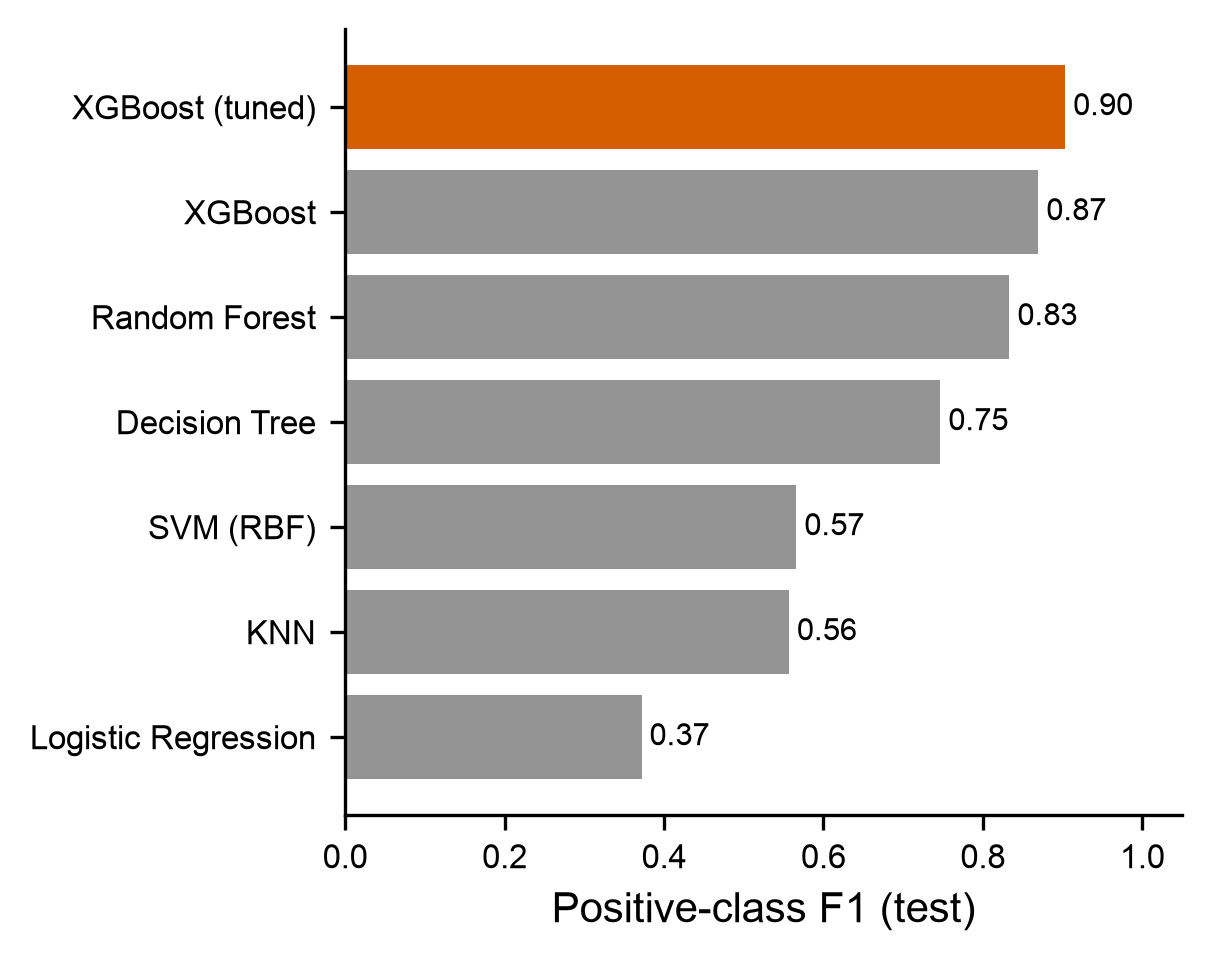
\includegraphics[width=\textwidth]{figures/model_comparison_f1.png}
\caption{}
\end{subfigure}
\hfill
\begin{subfigure}[t]{0.48\textwidth}
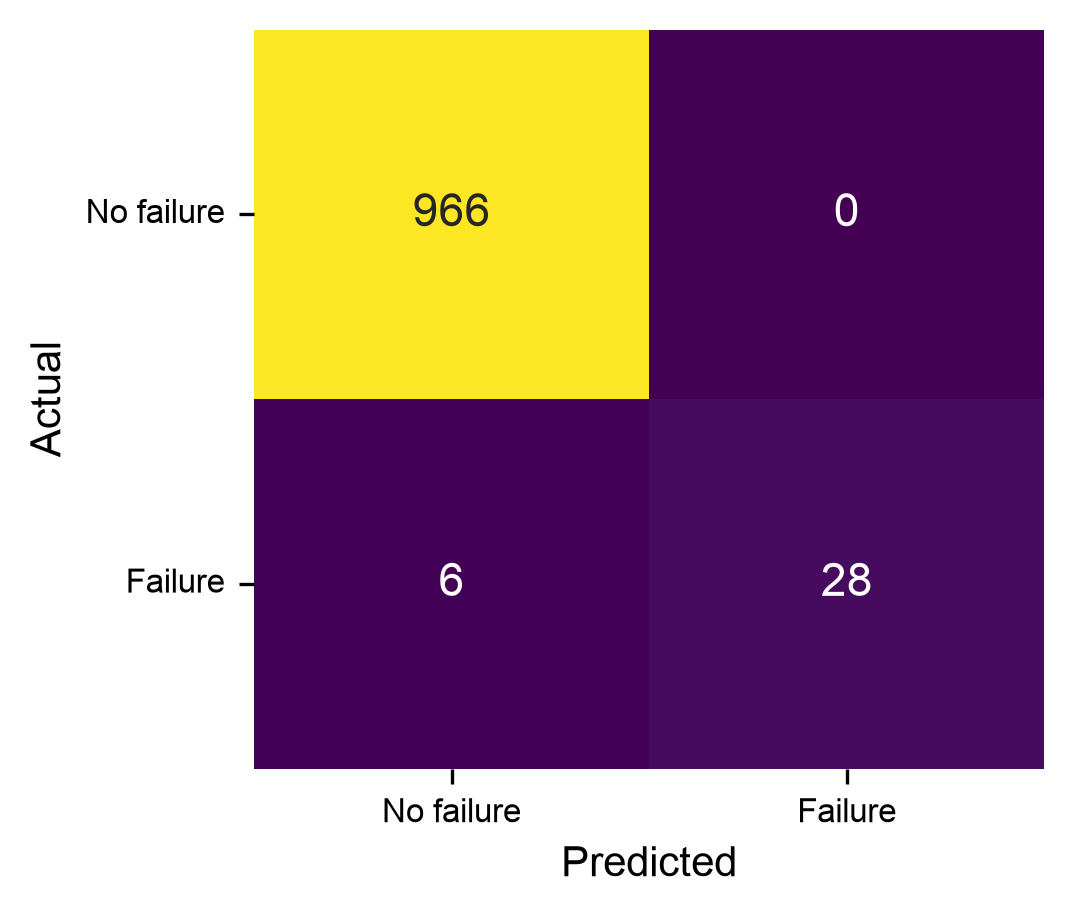
\includegraphics[width=\textwidth]{figures/confusion_matrix_best.png}
\caption{}
\end{subfigure}

\begin{subfigure}[t]{0.48\textwidth}

\includegraphics[width=\textwidth]{figures/roc_curves.png}
\caption{}
\end{subfigure}
\hfill
\begin{subfigure}[t]{0.48\textwidth}

\includegraphics[width=\textwidth]{figures/pr_curves.png}
\caption{}
\end{subfigure}
\caption{Test-set performance profile of the winning model. (a) Positive-class F1 across all
classical models (tuned XGBoost highlighted). (b) Confusion matrix for the tuned model at its
selected threshold. (c) ROC and (d) precision-recall curves for all classical models, tuned XGBoost
highlighted. The PyTorch MLP is omitted from (a), (c), (d) for legibility -- its numbers are in
Table~\ref{tab:models}.}
\label{fig:model-performance}
\end{figure}

Five-fold cross-validation of the tuned model (default 0.5 threshold per fold, hyperparameters
fixed) gives F1 $= 0.784 \pm 0.029$, precision $= 0.740 \pm 0.066$, recall $= 0.838 \pm 0.028$ --
confirming the single-split test result is not an artifact of a favorable split, and giving a more
conservative estimate than the threshold-tuned single-split number in Table~\ref{tab:models} (the
per-fold threshold was left at 0.5 deliberately, to isolate the model's raw discriminative behavior
from the threshold-tuning step).

\begin{table}[htbp]
\centering
\caption{Comparison against prior AI4I~2020 benchmarks. Metric definitions are not identical across
studies (macro-F1 averages both classes; positive-class F1 reports the failure class alone, which
is substantially harder under 3.39\% prevalence) -- we report both where available rather than
force a single number.}
\label{tab:priorwork}
\begin{tabular}{@{}llrl@{}}
\toprule
Study & Model & Metric & Value \\
\midrule
\citet{physicsinformed2026} & Random Forest & positive-class F1 & 0.722 \\
\citet{connectedvehicles2026} & LightGBM (5-fold CV, SMOTE in-fold) & macro-F1 & $0.814 \pm 0.012$ \\
This work & XGBoost (tuned, single split) & positive-class F1 & \textbf{0.90} \\
This work & XGBoost (tuned, single split) & macro-F1 & \textbf{0.95} \\
This work & XGBoost (tuned, 5-fold CV) & positive-class F1 & $0.784 \pm 0.029$ \\
\bottomrule
\end{tabular}
\end{table}

\subsection{Resampling comparison and decision boundaries}
Table~\ref{tab:resamplers} shows the validation-set bake-off; Borderline-SMOTE wins on F1 and is
used throughout. Figure~\ref{fig:decision-boundary} visualizes the effect directly: a Logistic
Regression classifier is fit on a 2D PCA projection of the training data, once per resampler. Without
resampling, the decision boundary barely bends toward the minority class; each oversampler pulls it
further into majority territory, visibly trading precision for recall -- the same tradeoff
Table~\ref{tab:models} shows numerically for the full feature space and stronger models.

\begin{table}[htbp]
\centering
\caption{Resampling technique comparison, validation set, fixed default XGBoost.}
\label{tab:resamplers}
\begin{tabular}{@{}lrrrr@{}}
\toprule
Sampler & Precision & Recall & F1 & PR-AUC \\
\midrule
\textbf{Borderline-SMOTE} & 0.814 & 0.838 & \textbf{0.826} & 0.883 \\
SMOTE                     & 0.699 & 0.853 & 0.768 & 0.892 \\
ADASYN                    & 0.683 & 0.824 & 0.747 & 0.876 \\
\bottomrule
\end{tabular}
\end{table}

\begin{figure}[htbp]
\centering

\includegraphics[width=0.95\textwidth]{figures/decision_boundary_2d.png}
\caption{Logistic Regression decision boundary in 2D PCA space, by sampling technique. Without
resampling the boundary is almost entirely majority-class; each oversampler shifts it toward the
minority region.}
\label{fig:decision-boundary}
\end{figure}

\subsection{Dimensionality reduction}
\label{sec:dimred}
The engineered features are not redundant: Figure~\ref{fig:pca-elbow} shows the PCA explained-variance
elbow, and 5 of the 12 processed features are needed to reach 95\% cumulative variance, so there is
little to compress away by design -- consistent with each engineered feature capturing a distinct
mechanism (Table~\ref{tab:mechanisms}) rather than a redundant transformation of the others.

\begin{figure}[htbp]
\centering
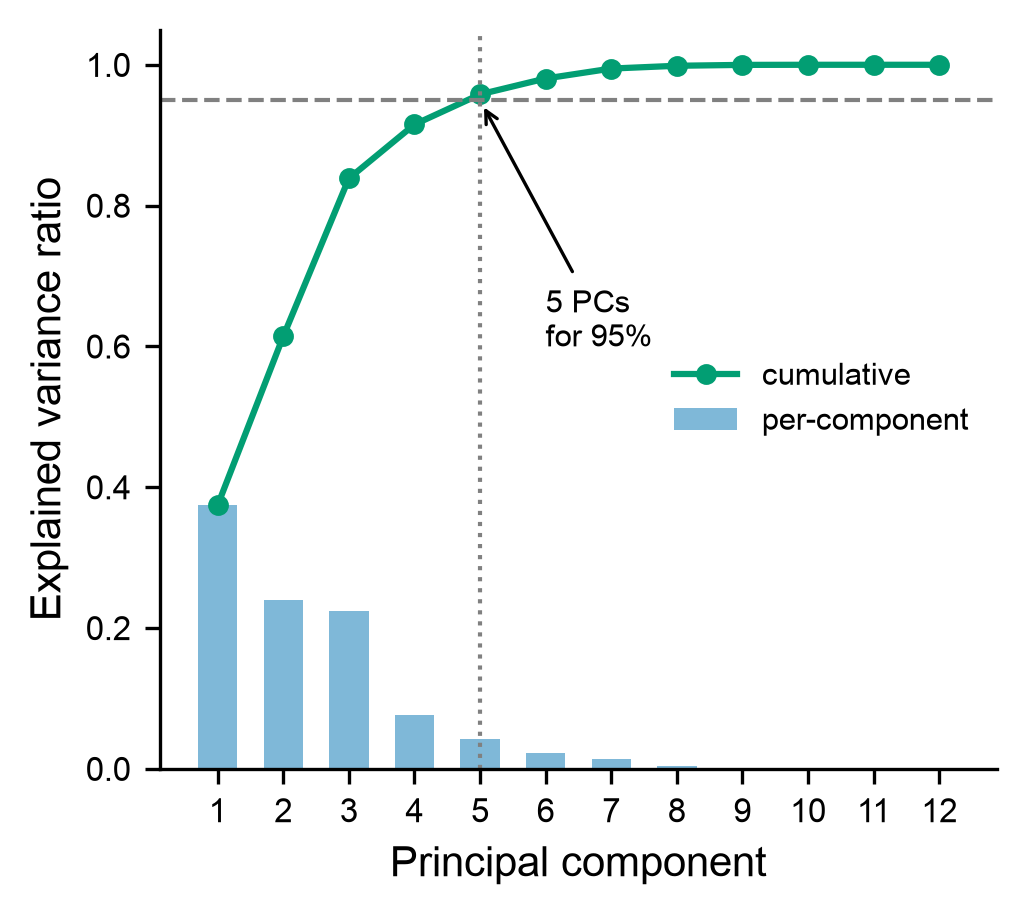
\includegraphics[width=0.42\textwidth]{figures/pca_elbow.png}
\caption{PCA explained-variance elbow on the processed training features. 5 of 12 components are
needed for 95\% cumulative variance.}
\label{fig:pca-elbow}
\end{figure}

Figure~\ref{fig:dimred} projects the training data into 2D with PCA, t-SNE \citep{vandermaaten2008tsne},
and UMAP \citep{mcinnes2018umap}. PCA (linear) shows the two classes smeared together with no
separating direction, consistent with linear models' weak performance in Table~\ref{tab:models}.
Both nonlinear methods instead show failure points clustering into several distinct pockets rather
than one contiguous region -- consistent with \texttt{Machine failure} being an aggregate of five
mechanistically distinct causes rather than a single failure mode with one shared signature.

\begin{figure}[htbp]
\centering

\includegraphics[width=0.95\textwidth]{figures/dimred_comparison.png}
\caption{PCA vs.\ t-SNE vs.\ UMAP projections of the training data, colored by \texttt{Machine
failure}.}
\label{fig:dimred}
\end{figure}

t-SNE cluster shape and spacing can be an artifact of the perplexity parameter rather than a
property of the data \citep{wattenberg2016misread}, so Figure~\ref{fig:tsne-perplexity} reruns
t-SNE on the same training data at perplexity $\in \{5, 30, 50, 100\}$. The failure points
consistently fall into the same right-side region of the embedding across all four settings --
the pocket structure in Figure~\ref{fig:dimred} is not a one-off artifact of the perplexity=30
default used there.

\begin{figure}[htbp]
\centering
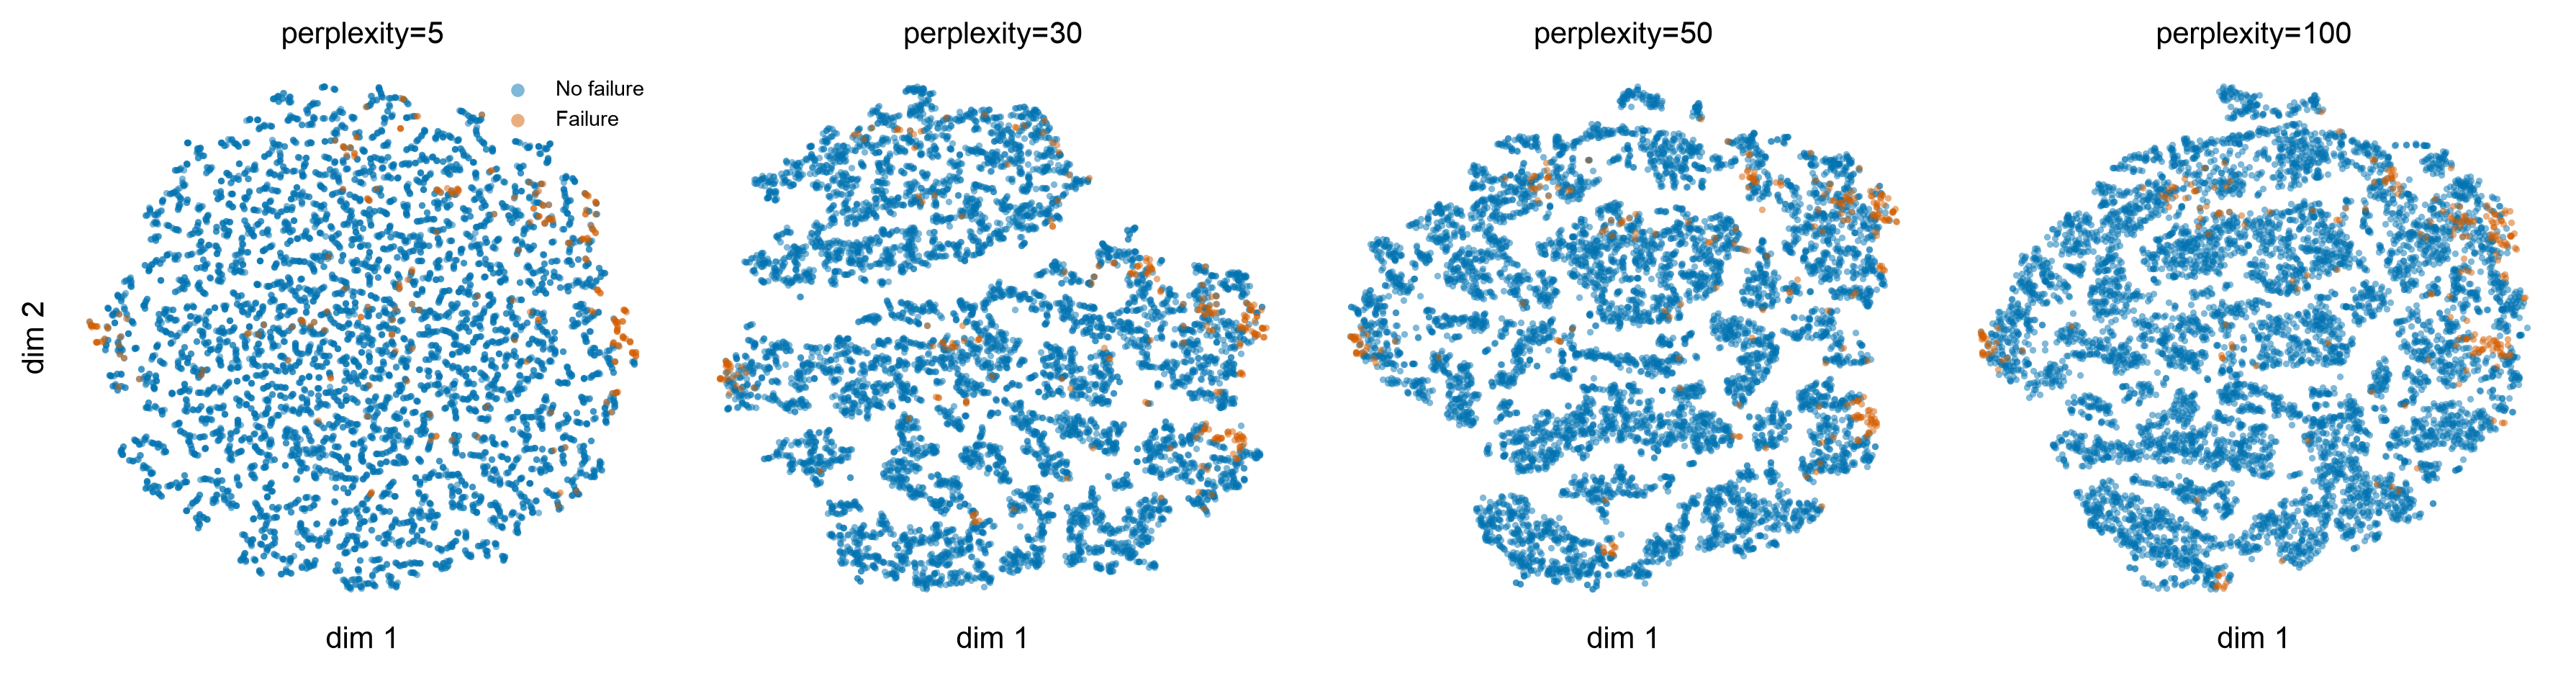
\includegraphics[width=0.95\textwidth]{figures/tsne_perplexity.png}
\caption{t-SNE embeddings of the training data at increasing perplexity. Failure points (orange)
occupy a consistent region of the embedding at every setting.}
\label{fig:tsne-perplexity}
\end{figure}

\subsection{XAI cross-check}
Table~\ref{tab:crosscheck} reports the outcome of the protocol in Section~\ref{sec:crosscheck}. All
five mechanisms pass: the model's top attributed feature for each of TWF, HDF, PWF, and OSF matches
that mechanism's known physical driver, and for RNF no single feature accounts for more than 17\% of
total subgroup attribution (below the 0.35 threshold), consistent with the fact that random failure
has no learnable cause. Figure~\ref{fig:shap-heatmap} shows the full per-feature,
per-mechanism attribution heatmap underlying this table, and Figure~\ref{fig:shap-summary} shows the
global SHAP summary for context.

\begin{table}[htbp]
\centering
\caption{XAI cross-check: does the model's top SHAP-attributed feature, restricted to rows where
mechanism $m$ fired, match $m$'s known physical cause?}
\label{tab:crosscheck}
\begin{tabular}{@{}llll@{}}
\toprule
Mechanism & Top attributed feature & Known cause & Result \\
\midrule
TWF & Tool wear [min] & Tool wear & \checkmark \\
HDF & Rotational speed [rpm] & Temp.\ gap / rotational speed & \checkmark \\
PWF & Power [W] & Torque $\times$ rpm & \checkmark \\
OSF & Overstrain\_ratio & Tool wear $\times$ torque & \checkmark \\
RNF & (none dominant, top share 0.17) & none -- pure chance & \checkmark \\
\bottomrule
\end{tabular}
\end{table}

\begin{figure}[htbp]
\centering

\includegraphics[width=0.85\textwidth]{figures/shap_crosscheck_heatmap.png}
\caption{Mean $|$SHAP value$|$ per feature, restricted to the rows where each mechanism fired.}
\label{fig:shap-heatmap}
\end{figure}

\begin{figure}[htbp]
\centering

\includegraphics[width=0.85\textwidth]{figures/shap_summary.png}
\caption{Global SHAP summary for the tuned model over the full dataset.}
\label{fig:shap-summary}
\end{figure}

\section{Discussion}

\subsection{What a failed audit would have shown}
Had the model instead attributed, say, Tool wear as the dominant feature for HDF rows, that would
indicate the classifier had latched onto a correlate of heat-dissipation failure (perhaps because
HDF and TWF co-occur more than chance in this particular data split) rather than the actual
temperature/speed mechanism -- a case where the model could still score well on held-out data while
being wrong about \emph{why}, a distinction that plain accuracy or even SHAP summary plots alone
would not surface. The RNF negative control is what makes the audit meaningful rather than
tautological: without it, a protocol that always finds \emph{some} top feature for every subgroup
provides no evidence of discriminating validity.

\subsection{Limitations}
\label{sec:limitations}
AI4I~2020 is a synthetic dataset generated from the same closed-form rules used as our ground truth
(Table~\ref{tab:mechanisms}); the ``ground truth'' is therefore the simulator's logic, not an
independently verified physical measurement from real equipment. This is a genuine limitation for
any claim that the protocol validates \emph{real-world} causal faithfulness, and we do not make that
claim here -- our contribution is the protocol and its demonstration, not a validated causal
finding about real machinery. This concern is not merely theoretical: \citet{autran2024ai4ipmdi}
show that injecting realistic irregularities (missing data, irregular time-series sampling) into
AI4I~2020 measurably changes downstream model performance, underscoring that results on the clean
synthetic version -- ours included -- may not transfer directly to messier real deployments. RNF
(19 rows total dataset-wide) and TWF (46 rows) are small enough
that per-mechanism subgroup SHAP estimates carry non-trivial variance; we mitigate this by computing
attributions over the full dataset rather than a single split, but a larger or non-synthetic
multi-mechanism dataset would give a more convincing demonstration. Finally, the audit as described
requires sub-labels for at least a validation subset of failures -- available here by construction,
and available in many industrial settings where maintenance logs record root cause even when the
model is only asked to predict binary failure, but not universal.

\subsection{Generalizability}
The protocol requires only two things: (1) a classifier trained on a coarse target, and (2) a
held-out set of finer-grained sub-labels for at least some of the positive cases, not used in
training. Both conditions are common in industrial PdM: maintenance tickets are frequently logged
with a root-cause code even when the deployed model only predicts a binary failure risk. In that
setting, this protocol offers a cheap, dataset-native alternative to constructing synthetic
ground-truth benchmarks purely to evaluate explanation faithfulness.

\section{Conclusion}
We show that AI4I~2020's five failure mechanisms, ordinarily discarded once the composite failure
label is formed, can be repurposed as a faithfulness probe for post-hoc SHAP explanations. A tuned
XGBoost classifier trained only on the composite label attributes each of four real mechanisms to
its correct physical driver and shows no dominant feature for the one mechanism with no real cause.
Beyond the specific result, we position this as a general, low-cost protocol applicable wherever a
coarse PdM target aggregates several distinct, partially-labeled failure modes -- the common case in
practice -- as a complement to, not a replacement for, existing faithfulness-evaluation methods built
on purpose-designed synthetic data.

\bibliographystyle{plainnat}
\bibliography{refs}

\end{document}
